%%%%%%%% ICML 2024 EXAMPLE LATEX SUBMISSION FILE %%%%%%%%%%%%%%%%%

\documentclass{article}

% Recommended, but optional, packages for figures and better typesetting:
\usepackage{microtype}
\usepackage{graphicx}
\usepackage{subfigure}
\usepackage{booktabs} % for professional tables

% hyperref makes hyperlinks in the resulting PDF.
% If your build breaks (sometimes temporarily if a hyperlink spans a page)
% please comment out the following usepackage line and replace
% \usepackage{icml2024} with \usepackage[nohyperref]{icml2024} above.
\usepackage{hyperref}


% Attempt to make hyperref and algorithmic work together better:
\newcommand{\theHalgorithm}{\arabic{algorithm}}

% Use the following line for the initial blind version submitted for review:
\usepackage{icml2024}

% If accepted, instead use the following line for the camera-ready submission:
% \usepackage[accepted]{icml2024}

% For theorems and such
\usepackage{amsmath}
\usepackage{amssymb}
\usepackage{mathtools}
\usepackage{amsthm}

% if you use cleveref..
\usepackage[capitalize,noabbrev]{cleveref}

%%%%%%%%%%%%%%%%%%%%%%%%%%%%%%%%
% THEOREMS
%%%%%%%%%%%%%%%%%%%%%%%%%%%%%%%%
\theoremstyle{plain}
\newtheorem{theorem}{Theorem}[section]
\newtheorem{proposition}[theorem]{Proposition}
\newtheorem{lemma}[theorem]{Lemma}
\newtheorem{corollary}[theorem]{Corollary}
\theoremstyle{definition}
\newtheorem{definition}[theorem]{Definition}
\newtheorem{assumption}[theorem]{Assumption}
\theoremstyle{remark}
\newtheorem{remark}[theorem]{Remark}

% Todonotes is useful during development; simply uncomment the next line
%    and comment out the line below the next line to turn off comments
%\usepackage[disable,textsize=tiny]{todonotes}
\usepackage[textsize=tiny]{todonotes}


% The \icmltitle you define below is probably too long as a header.
% Therefore, a short form for the running title is supplied here:
\icmltitlerunning{Sample-efficient Reinforcement Learning with Latent Representations}

%%%%%%%%%%%%%%%%%%%%%%%%%%%%%%%%
% CUSTOM (our stuff)
%%%%%%%%%%%%%%%%%%%%%%%%%%%%%%%%

\newcommand{\our}{\textsc{vq-td3}\xspace}

% Latin
\usepackage{xspace}
\newcommand{\eg}{\textit{e.g.\@}\xspace}
\newcommand{\ie}{\textit{i.e.\@}\xspace}
\newcommand{\cf}{\textit{cf.\@}\xspace}
\newcommand{\etc}{\textit{etc.\@}\xspace}
\newcommand{\etal}{\textit{et~al.\@}\xspace}

% Vectors
\def\vzero{{\bm{0}}}
\def\vone{{\bm{1}}}
\def\vmu{{\bm{\mu}}}
\def\vtheta{{\bm{\theta}}}
\def\va{{\bm{a}}}
\def\vb{{\bm{b}}}
\def\vc{{\bm{c}}}
\def\vd{{\bm{d}}}
\def\ve{{\bm{e}}}
\def\vf{{\bm{f}}}
\def\vg{{\bm{g}}}
\def\vh{{\bm{h}}}
\def\vi{{\bm{i}}}
\def\vj{{\bm{j}}}
\def\vk{{\bm{k}}}
\def\vl{{\bm{l}}}
\def\vm{{\bm{m}}}
\def\vn{{\bm{n}}}
\def\vo{{\bm{o}}}
\def\vp{{\bm{p}}}
\def\vq{{\bm{q}}}
\def\vr{{\bm{r}}}
\def\vs{{\bm{s}}}
\def\vt{{\bm{t}}}
\def\vu{{\bm{u}}}
\def\vv{{\bm{v}}}
\def\vw{{\bm{w}}}
\def\vx{{\bm{x}}}
\def\vy{{\bm{y}}}
\def\vz{{\bm{z}}}

% Elements of vectors
\def\evalpha{{\alpha}}
\def\evbeta{{\beta}}
\def\evepsilon{{\epsilon}}
\def\evlambda{{\lambda}}
\def\evomega{{\omega}}
\def\evmu{{\mu}}
\def\evpsi{{\psi}}
\def\evsigma{{\sigma}}
\def\evtheta{{\theta}}
\def\eva{{a}}
\def\evb{{b}}
\def\evc{{c}}
\def\evd{{d}}
\def\eve{{e}}
\def\evf{{f}}
\def\evg{{g}}
\def\evh{{h}}
\def\evi{{i}}
\def\evj{{j}}
\def\evk{{k}}
\def\evl{{l}}
\def\evm{{m}}
\def\evn{{n}}
\def\evo{{o}}
\def\evp{{p}}
\def\evq{{q}}
\def\evr{{r}}
\def\evs{{s}}
\def\evt{{t}}
\def\evu{{u}}
\def\evv{{v}}
\def\evw{{w}}
\def\evx{{x}}
\def\evy{{y}}
\def\evz{{z}}

% Matrix
\def\mA{{\bm{A}}}
\def\mB{{\bm{B}}}
\def\mC{{\bm{C}}}
\def\mD{{\bm{D}}}
\def\mE{{\bm{E}}}
\def\mF{{\bm{F}}}
\def\mG{{\bm{G}}}
\def\mH{{\bm{H}}}
\def\mI{{\bm{I}}}
\def\mJ{{\bm{J}}}
\def\mK{{\bm{K}}}
\def\mL{{\bm{L}}}
\def\mM{{\bm{M}}}
\def\mN{{\bm{N}}}
\def\mO{{\bm{O}}}
\def\mP{{\bm{P}}}
\def\mQ{{\bm{Q}}}
\def\mR{{\bm{R}}}
\def\mS{{\bm{S}}}
\def\mT{{\bm{T}}}
\def\mU{{\bm{U}}}
\def\mV{{\bm{V}}}
\def\mW{{\bm{W}}}
\def\mX{{\bm{X}}}
\def\mY{{\bm{Y}}}
\def\mZ{{\bm{Z}}}
\def\mBeta{{\bm{\beta}}}
\def\mPhi{{\bm{\Phi}}}
\def\mLambda{{\bm{\Lambda}}}
\def\mSigma{{\bm{\Sigma}}}

\newcommand{\E}{\mathbb{E}}
\newcommand{\Ls}{\mathcal{L}}
\newcommand{\R}{\mathbb{R}}
\newcommand{\emp}{\tilde{p}}
\newcommand{\lr}{\alpha}
\newcommand{\reg}{\lambda}
\newcommand{\rect}{\mathrm{rectifier}}
\newcommand{\softmax}{\mathrm{softmax}}
\newcommand{\sigmoid}{\sigma}
\newcommand{\softplus}{\zeta}
\newcommand{\KL}{D_{\mathrm{KL}}}
\newcommand{\Var}{\mathrm{Var}}
\newcommand{\standarderror}{\mathrm{SE}}
\newcommand{\Cov}{\mathrm{Cov}}
% Wolfram Mathworld says $L^2$ is for function spaces and $\ell^2$ is for vectors
% But then they seem to use $L^2$ for vectors throughout the site, and so does
% wikipedia.
\newcommand{\normlzero}{L^0}
\newcommand{\normlone}{L^1}
\newcommand{\normltwo}{L^2}
\newcommand{\normlp}{L^p}
\newcommand{\normmax}{L^\infty}

\DeclareMathOperator*{\argmax}{arg\,max}
\DeclareMathOperator*{\argmin}{arg\,min}

%%%%%%%%%%%%%%%%%%%%%%%%%%%%%%%%
% BEGIN DOCUMENT
%%%%%%%%%%%%%%%%%%%%%%%%%%%%%%%%
\begin{document}

\twocolumn[
% \icmltitle{Submission and Formatting Instructions for \\
%            International Conference on Machine Learning (ICML 2024)}
\icmltitle{Sample-efficient Reinforcement Learning with Latent Representations}

% It is OKAY to include author information, even for blind
% submissions: the style file will automatically remove it for you
% unless you've provided the [accepted] option to the icml2024
% package.

% List of affiliations: The first argument should be a (short)
% identifier you will use later to specify author affiliations
% Academic affiliations should list Department, University, City, Region, Country
% Industry affiliations should list Company, City, Region, Country

% You can specify symbols, otherwise they are numbered in order.
% Ideally, you should not use this facility. Affiliations will be numbered
% in order of appearance and this is the preferred way.
\icmlsetsymbol{equal}{*}

\begin{icmlauthorlist}
\icmlauthor{Aidan Scannell}{aalto,fcai}
\icmlauthor{Arno Solin}{aalto}
\icmlauthor{Joni Pajarinen}{aalto}
% \icmlauthor{Firstname1 Lastname1}{equal,yyy}
% \icmlauthor{Firstname2 Lastname2}{equal,yyy,comp}
% \icmlauthor{Firstname3 Lastname3}{comp}
% \icmlauthor{Firstname4 Lastname4}{sch}
% \icmlauthor{Firstname5 Lastname5}{yyy}
% \icmlauthor{Firstname6 Lastname6}{sch,yyy,comp}
% \icmlauthor{Firstname7 Lastname7}{comp}
% %\icmlauthor{}{sch}
% \icmlauthor{Firstname8 Lastname8}{sch}
% \icmlauthor{Firstname8 Lastname8}{yyy,comp}
%\icmlauthor{}{sch}
%\icmlauthor{}{sch}
\end{icmlauthorlist}

\icmlaffiliation{aalto}{Aalto University, Finland}
\icmlaffiliation{fcai}{Finnish Center for Artificial Intelligence}
% \icmlaffiliation{yyy}{Department of XXX, University of YYY, Location, Country}
% \icmlaffiliation{comp}{Company Name, Location, Country}
% \icmlaffiliation{sch}{School of ZZZ, Institute of WWW, Location, Country}

\icmlcorrespondingauthor{Aidan Scannell}{aidan.scannell@aalto.fi}
% \icmlcorrespondingauthor{Firstname1 Lastname1}{first1.last1@xxx.edu}
% \icmlcorrespondingauthor{Firstname2 Lastname2}{first2.last2@www.uk}

% You may provide any keywords that you
% find helpful for describing your paper; these are used to populate
% the "keywords" metadata in the PDF but will not be shown in the document
\icmlkeywords{Machine Learning, ICML}

\vskip 0.3in
]

% this must go after the closing bracket ] following \twocolumn[ ...

% This command actually creates the footnote in the first column
% listing the affiliations and the copyright notice.
% The command takes one argument, which is text to display at the start of the footnote.
% The \icmlEqualContribution command is standard text for equal contribution.
% Remove it (just {}) if you do not need this facility.

\printAffiliationsAndNotice{}  % leave blank if no need to mention equal contribution
% \printAffiliationsAndNotice{\icmlEqualContribution} % otherwise use the standard text.

\begin{abstract}
This document provides a basic paper template and submission guidelines.
Abstracts must be a single paragraph, ideally between 4--6 sentences long.
Gross violations will trigger corrections at the camera-ready phase.
\end{abstract}


\section{Introduction}
\label{intro}

Reinforcement learning (RL) has potential...

However, applying RL in real-world environments with high dimensional/complex observation spaces is challenging.

Compressing observations in latent state space.
Hand crafted features

Learning features with representation learning.
These methods typically learn task-specific representations
as they train the representation to predict rewards and/or values
\citep{zhaoSimplifiedTemporalConsistency2023,hansenTemporalDifferenceLearning2022}

For example, \citet{zhaoSimplifiedTemporalConsistency2023} use a latent-state consistency loss based upon the Cosine
similarity loss plus the MSE of reward predictions in the latent space.
The cosine similarity loss provides training stability whilst the reward prediction prevents representation collapse.

In this paper, we propose a simple representation learning technique that can be combined with any model-free RL method.
Normalization based upon Finite Scalar Quantization
Importantly, our representation {\em (i)} significantly speeds up learning, {\em (ii)} prevents representation collapse,
and {\em (iii)} is task-agnostic.

% In recent years, it has become common to

\begin{figure}[ht]
\vskip 0.2in
\begin{center}
\centerline{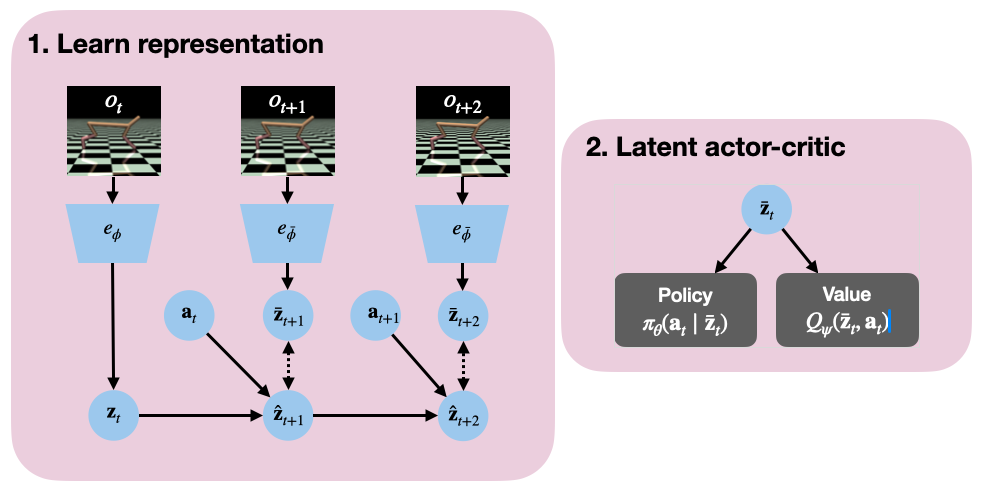
\includegraphics[width=\columnwidth]{./figs/method-diagram.png}}
\caption{Self-predictice loss}
\label{diagram-self-predictive}
\end{center}
\vskip -0.2in
\end{figure}



\section{Related Work}
\label{related_work}



\textbf{Sample-efficiency in deep RL}
Many approaches have been proposed to improve sample efficiency in deep RL.
As \citet{laskinCURLContrastiveUnsupervised2020} highlighted, these can generally be divided into two streams of research:
{\em (i)} auxillary tasks on the agent's observations and {\em (ii)} world models that predict the future
\citep{haRecurrentWorldModels2018,hafnerLearning2019,hansenTemporalDifferenceLearning2022}.
In this work, we are interested in the first class of methods, which use auxillary tasks to improve sample efficiency.

\textbf{Representation learning for RL}
Learning representations for RL has been investigated for decades
\citep{abelOptimalBehaviorApproximate2016,mannorDynamicAbstractionReinforcement2004,liUnifiedTheoryState2006,andreStateAbstractionProgrammable2002,deardenAbstractionApproximateDecisiontheoretic1997,singhReinforcementLearningSoft1994,higginsDefinitionDisentangledRepresentations2018,vanhoofStableReinforcementLearning2016,watterEmbedControlLocally2015,ghoshRepresentationsStableOffPolicy2020}.
However, these approaches are usually limited to simple environments.
Some approaches used unsupervised learning (\eg VAE \citep{kingmaAutoEncoding2014} with reconstruction loss) to acquire representations
\cite{finnDeepSpatialAutoencoders2016,higginsDARLAImprovingZeroShot2017,langeAutonomousReinforcementLearning2012,watterEmbedControlLocally2015}.
More recently, self-supervised learning (SSL) approaches (which do not reconstruct observations)
attempt to learn good features without labels \cite{anandUnsupervisedStateRepresentation2019}.
Alternative approaches leverage contrastive losses to learn representations \cite{laskinCURLContrastiveUnsupervised2020}.

\citet{yaratsImprovingSampleEfficiency2021} learn a compact representation with a deterministic autoencoder and then train a
SAC agent \citep{haarnojaSoft2018} with the representation. They name their method SAC-AE.
Interestingly, SAC-AE matches the performance of model-based methods like PlaNet \citep{hafnerLearning2019}
and SLAC \citep{leeStochasticLatentActorCritic2020}, whilst being considerably simpler to implement.

\textbf{Bisimulation}
DeepMDP \citep{geladaDeepMDPLearningContinuous2019},
deep bisimulation for control (DBC) \citep{zhangLearningInvariantRepresentations2020}
and DHGP \citep{rezaei-shoshtariContinuousMDPHomomorphisms2022}
% \citet{geladaDeepMDPLearningContinuous2019,zhangLearningInvariantRepresentations2020,rezaei-shoshtariContinuousMDPHomomorphisms2022}
use SSL losses based on bisimulation metrics \citep{larsenBisimulationProbabilisticTesting1989}.
As such, their encoders group states into clusters whilst preserving some properties
(\eg optimal value, all values, all action values from each state) \citep{liUnifiedTheoryState2006}.
These methods use latent-space dynamic models to learn latent representations which encode only task-relevant information.
% Interestingly, the dynamics models are only used for representation learning and are not used for model-based planning.
DeepMDP \citep{geladaDeepMDPLearningContinuous2019} combines its representation learning with
distributional Q learning  \citep[C51,][]{bellemareDistributionalPerspectiveReinforcement2017},
whilst DBC \citep{zhangLearningInvariantRepresentations2020} combine its method with SAC.


% \cite{zhaoSimplifiedTemporalConsistency2023}
% \cite{hansenTemporalDifferenceLearning2022}

% \cite{higginsDefinitionDisentangledRepresentations2018,vanhoofStableReinforcementLearning2016,watterEmbedControlLocally2015} use VAE \citep{kingmaAutoEncoding2014}

% \citet{zhangLearningInvariantRepresentations2020} to learn a latent representation which encode only
% task-relevant information.
% Their method is named deep bisimulation for control (DBC) and they combine their representation learning method with SAC.


\textbf{Primacy bias}
Primacy bias in deep RL \citep{nikishinPrimacyBiasDeep2022}
is where an agent overfits on early data and loses its ability to learn from new data,
which arises due to the plasticity in NNs \citep{lyleUnderstandingPlasticityNeural2023} \todo{earlier citation of plasticiy in NNs??}.
\citet{nikishinPrimacyBiasDeep2022} showed that periodically resetting the agent's parameters can help alleviate primacy bias.
\citet{doroSampleEfficientReinforcementLearning2022} built on top of this insight and showed that resetting the
agent's parameters not only alleviates primacy bias but also
enables the number of parameter update's per environment interaction to be increased.
They refer to this as the replay ratio but it has also been referred to as the update to data
ratio (UTD) \citep{chenRandomizedEnsembledDouble2021}.
\citet{nikishinDeepReinforcementLearning2023} propose an alternative approach to overcome primacy bias which
freezes the current NN and creates a new one which learns the changes in predictions.


When leveraging latent representations for RL (\eg SLAC \citep{leeStochasticLatentActorCritic2020},
SAC-AE \citep{yaratsImprovingSampleEfficiency2021}) this issue is exacerbated.
Not only do the agents networks (\eg actor/critic) overfit on early data, but as the encoder is updated during training, the
inputs (latent states) that the networks are trained on change.
As such, the networks are overfit on latent states which no longer exist in the ``latent'' data set.



\textbf{Misc}
\citet{obando-ceronSmallBatchDeep2023a} show that reducing the batch size not only improves
performance and wall-time gains, but also appears to have knock-on effects on exploration and asymptotic behaviour.

\citet{lyuOffPolicyRLAlgorithms2023} show that performing multiple parameter updates for a given batch.
Their method, name sample multiple reuse (SMR), improves sample efficiency
They say not to use if for image-based environments like Atari.


Simplical embeddings
\cite{lavoieSimplicialEmbeddingsSelfSupervised2022}


\section{Method}
\label{sec:method}

In this section, we detail our method, titled Vector Quantized TD3 (\our).
\our is conceptually simple, it first learns a representation of the observation space and then,
given this representation, it performs model-free RL (e.g. TD3) on this representation.
% It the first representation learning phase, it learns an encoder which maps observations $o \in \mathcal{O}$
% to a latent space $z \in \mathcal{Z}$.
% It first learns a representation of the observation space and then uses
See \cref{alg:main_alg}.

We consider Markov Decision Processes (MDPs, \citet{bellmanMarkovianDecisionProcess1957a}) $\mathcal{M} = (\mathcal{O}, \mathcal{A}, \mathcal{P}, \mathcal{R}, \gamma,\mathcal{T})$, where an agent receives
observation $o_{t} \in \mathcal{O}$ at time step $t$ and performs an action $a_{t} \in \mathcal{A}$.
The agent then obtains a reward $r_{t} = \mathcal{R} (o_{t}, a_{t})$ and obtains the next observation
$o_{t+1} = P(\cdot \mid o_{t}, a_{t})$.
discount factor $\gamma \in [0, 1]$


\our has four parameterized components.
\begin{algorithm}[tb]
   \caption{\our}
   \label{alg:main_alg}
\begin{algorithmic}
   \STATE {\bfseries Input:} Encoder $e_{\theta}$, transition $d_{\phi}$, critics $Q_{\psi}$, policy $\pi_{\eta}$
   \FOR{$i$ {\bfseries to} $N_{\text{episodes}}$}
    \STATE $\mathcal{D} \leftarrow \mathcal{D} \cup \{o_{t}, a_{t}, o_{t+1}, r_{t+1}\}^{T}_{t=0}$
    \FOR{$i=1$ {\bfseries to} $T \times UTD$}
        \STATE Representation update
        \STATE TD3 update
    \ENDFOR
   \ENDFOR
\end{algorithmic}
\end{algorithm}

\begin{align}
\text{Encoder: } &z_{t} = e_{\theta} (s_{t}) \label{eq:encoder} \\
\text{Dynamics: } &\hat{z}_{t+1} = d_{\phi} (z_{t}, a_{t}) \label{eq:transition} \\
\text{Value: } &q_{t} = Q_{\psi} (z_{t}, a_{t}) \label{eq:value} \\
\text{Policy: } &a_{t} \sim \pi_{\eta} (z_{t}) , \label{eq:policy}
\end{align}
Note that unlike TCRL \citep{zhaoSimplifiedTemporalConsistency2023}, our transition model does
not predict the reward.

\textbf{Representation learning}
Our representation learning is based soley on the temporal consistency loss,
However, unlike previous works, we normalize the latent vector
Our representation learning consists of an encoder $e_{\theta}$ (which maps observations to
latent states) and a transition model $d_{\phi}$ which maps
Our representation learning adopts a self-supervised loss.

\begin{align} \label{eq:rep-loss}
  \mathcal{L}_{\text{rep}}(\theta, \phi; \mathcal{D})
 % &= \E_{s_{t} \sim \mathcal{D}} \left[ \sum_{h=0}^{H-1} \| \hat{z}_{t+1} - z_{t+1} \|_{2}^{2} \right] \\
%&= \E_{(s_{t}, a_{t}, s_{t+1}) \sim \mathcal{D}}
&= \E_{\tau \sim \mathcal{D}}
\left[ \sum_{h=0}^{H-1} \gamma^{h} \| d_{\phi}(e_{\theta}(s_{t}), a_{t}) - e_{\bar{\theta}}(s_{t+1}) \|_{2}^{2} \right]
\end{align}

\textbf{Finite Scalar Quantization}
We follow Finite Scalar Quantization (FSQ, \cite{mentzerFiniteScalarQuantization2023})
and bound each dimension of our latent space.
Given the output of our MLP encoder $z \in \R^{d}$,

where each entry in  $f : z \rightarrow \left[ L/2 \right] \mathrm{tanh}(z))$

% Thereby, we have zˆ ∈ C, where C is the implied codebook, given by the product of these per-channel
% codebook sets, with |C| = L
% d
% . The vectors in C can simply be enumerated leading to a bijection from
% any zˆ to an integer in {1, . . . , Ld}. Therefore, VQ can be replaced with FSQ in any neural networkrelated setup where VQ is commonly used, e.g., to train transformers, after appropriately adapting
% the output and input dimension of the layers before and after VQ, respectively. We generalize the
% above exposition to the case where the i-th channel is mapped to Li values and get |C| =
% Qd
% i=1 Li


\textbf{Policy and value function learning}

\begin{align} \label{eq:value-loss}
  \mathcal{L}_{Q}(\psi ; \mathcal{D}) &= \E_{\tau \sim \mathcal{D}} \left[ (Q_{\psi_{k}}(e_{\theta}(s_{t}), a_{t}) - y)^{2}  \right], \quad \forall k \in 1, 2 \\
  y &= \sum_{n=0}^{N-1} \gamma^{n} r_{t+n} + \gamma^{n} \min_{k \in \{1,2\}} Q_{\bar{\psi}_{k}}(e_{\bar{\theta}}(s_{t+n}), a_{t+n})
\end{align}


\begin{align} \label{eq:policy-loss}
 \mathcal{L}_{\pi}(\eta; \mathcal{D}) = \E_{(o_{t}, a_{t}) \sim \mathcal{D}} \left[ \min_{k\in\{1,2\}} Q_{\psi_{k}}(e_{\theta}(o_{t}), a_{t}) \right]
\end{align}

\section{Experiments}
\label{sec:experiments}

\begin{table}[t]
\caption{FSQ levels $\mathcal{L}$ to approximate different codebook sizes $|\mathcal{C}|$}
\label{sample-table}
\vskip 0.15in
\begin{center}
\begin{small}
\begin{sc}
\begin{tabular}{lccc}
\toprule
Target size $|\mathcal{C}|$ & $2^{8}$ & $2^{10}$ & $2^{12}$ \\
\midrule
Proposed $\mathcal{L}$ & $[8,6,5]$ & $[8,5,5,5]$ & $[7,5,5,5,5]$ \\
% \bottomrule
\end{tabular}
\end{sc}
\end{small}
\end{center}
\vskip -0.1in
\end{table}


\begin{figure*}[ht]
\vskip 0.2in
\begin{center}
\centerline{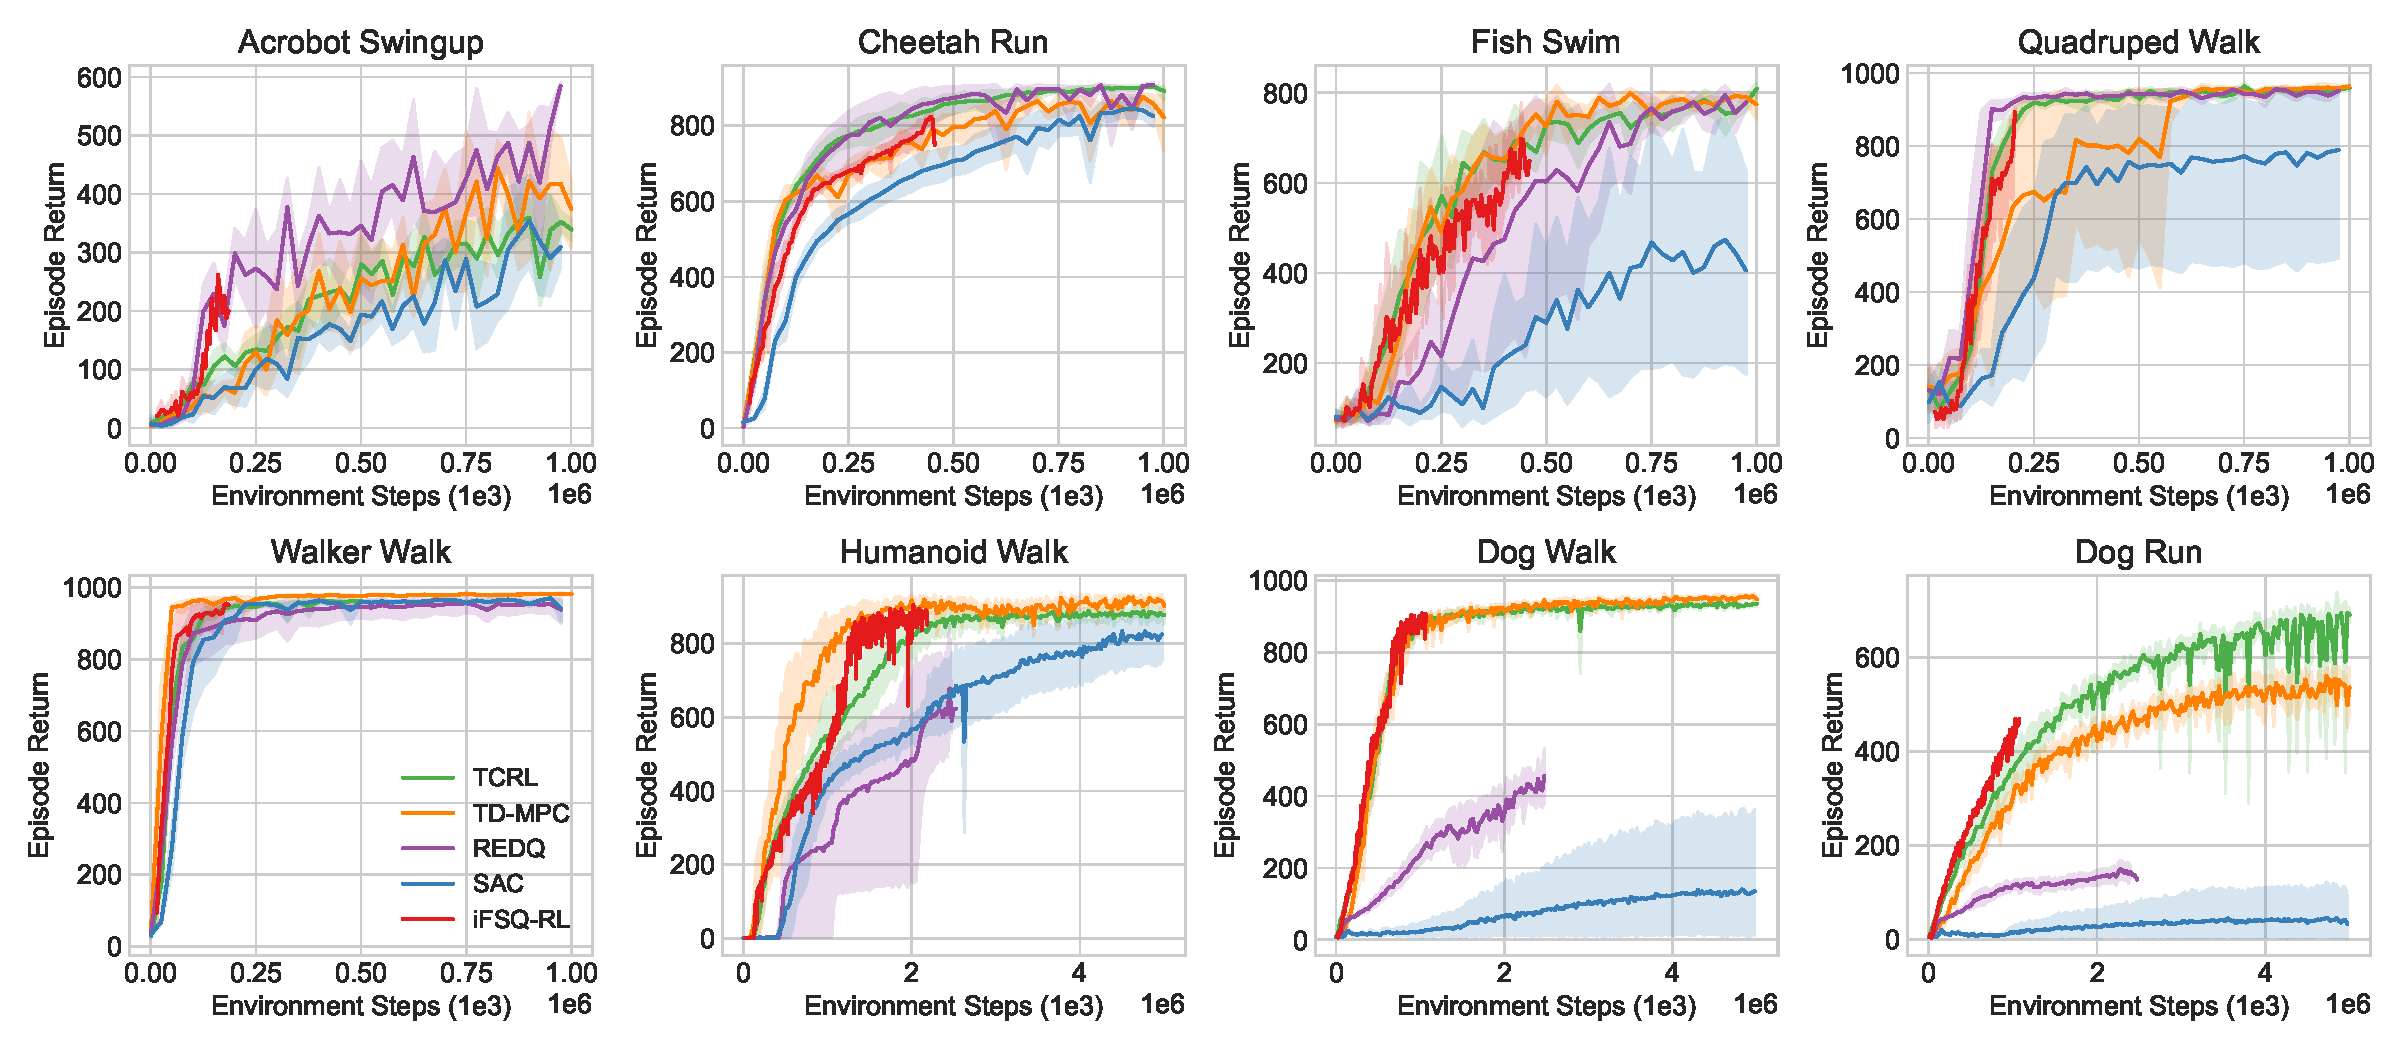
\includegraphics[width=1.0\textwidth]{./figs/main_plot.pdf}}
\caption{Comparison to baselines with UTD=1.}
\label{fig:main_plot}
\end{center}
\vskip -0.2in
\end{figure*}


\begin{itemize}
    \item Show normalised latent leads to higher sample efficiency. Show results for NTC-TD3/TC-TD3/TD3/SAC/TCRL/TD-MPC with UTD=1.
    \item Show normalised latent works with higher UTD. Compare NTC-TD3/TC-TD3/TCRL.
    \item Show task-agnostic representation is good for incremental task learning. Compare NTC-TD3/TCRL-ours/TCRL
\end{itemize}

\text{Ablations}



\begin{itemize}
  \item Show un-normalised isn't as good.
  \item Compare different size latent spaces? Different levels $[8,5]$ vs $[8,6,5]$ vs $[8,5,5,5]$ vs $[7,5,5,5,5]$
  \item Target encoder vs online encoder for mapping states to latents for TD3.
  \item Show cosine similarity slows training.
  \item Show adding reconstruction loss hurts performance.
\end{itemize}







\section{Conclusion}
\label{conclusion}

% In the unusual situation where you want a paper to appear in the
% references without citing it in the main text, use \nocite

\bibliography{zotero-library}
\bibliographystyle{icml2024}


%%%%%%%%%%%%%%%%%%%%%%%%%%%%%%%%%%%%%%%%%%%%%%%%%%%%%%%%%%%%%%%%%%%%%%%%%%%%%%%
%%%%%%%%%%%%%%%%%%%%%%%%%%%%%%%%%%%%%%%%%%%%%%%%%%%%%%%%%%%%%%%%%%%%%%%%%%%%%%%
% APPENDIX
%%%%%%%%%%%%%%%%%%%%%%%%%%%%%%%%%%%%%%%%%%%%%%%%%%%%%%%%%%%%%%%%%%%%%%%%%%%%%%%
%%%%%%%%%%%%%%%%%%%%%%%%%%%%%%%%%%%%%%%%%%%%%%%%%%%%%%%%%%%%%%%%%%%%%%%%%%%%%%%
\newpage
\appendix
\onecolumn
\section{You \emph{can} have an appendix here.}

\begin{figure*}[ht]
\vskip 0.2in
\begin{center}
\centerline{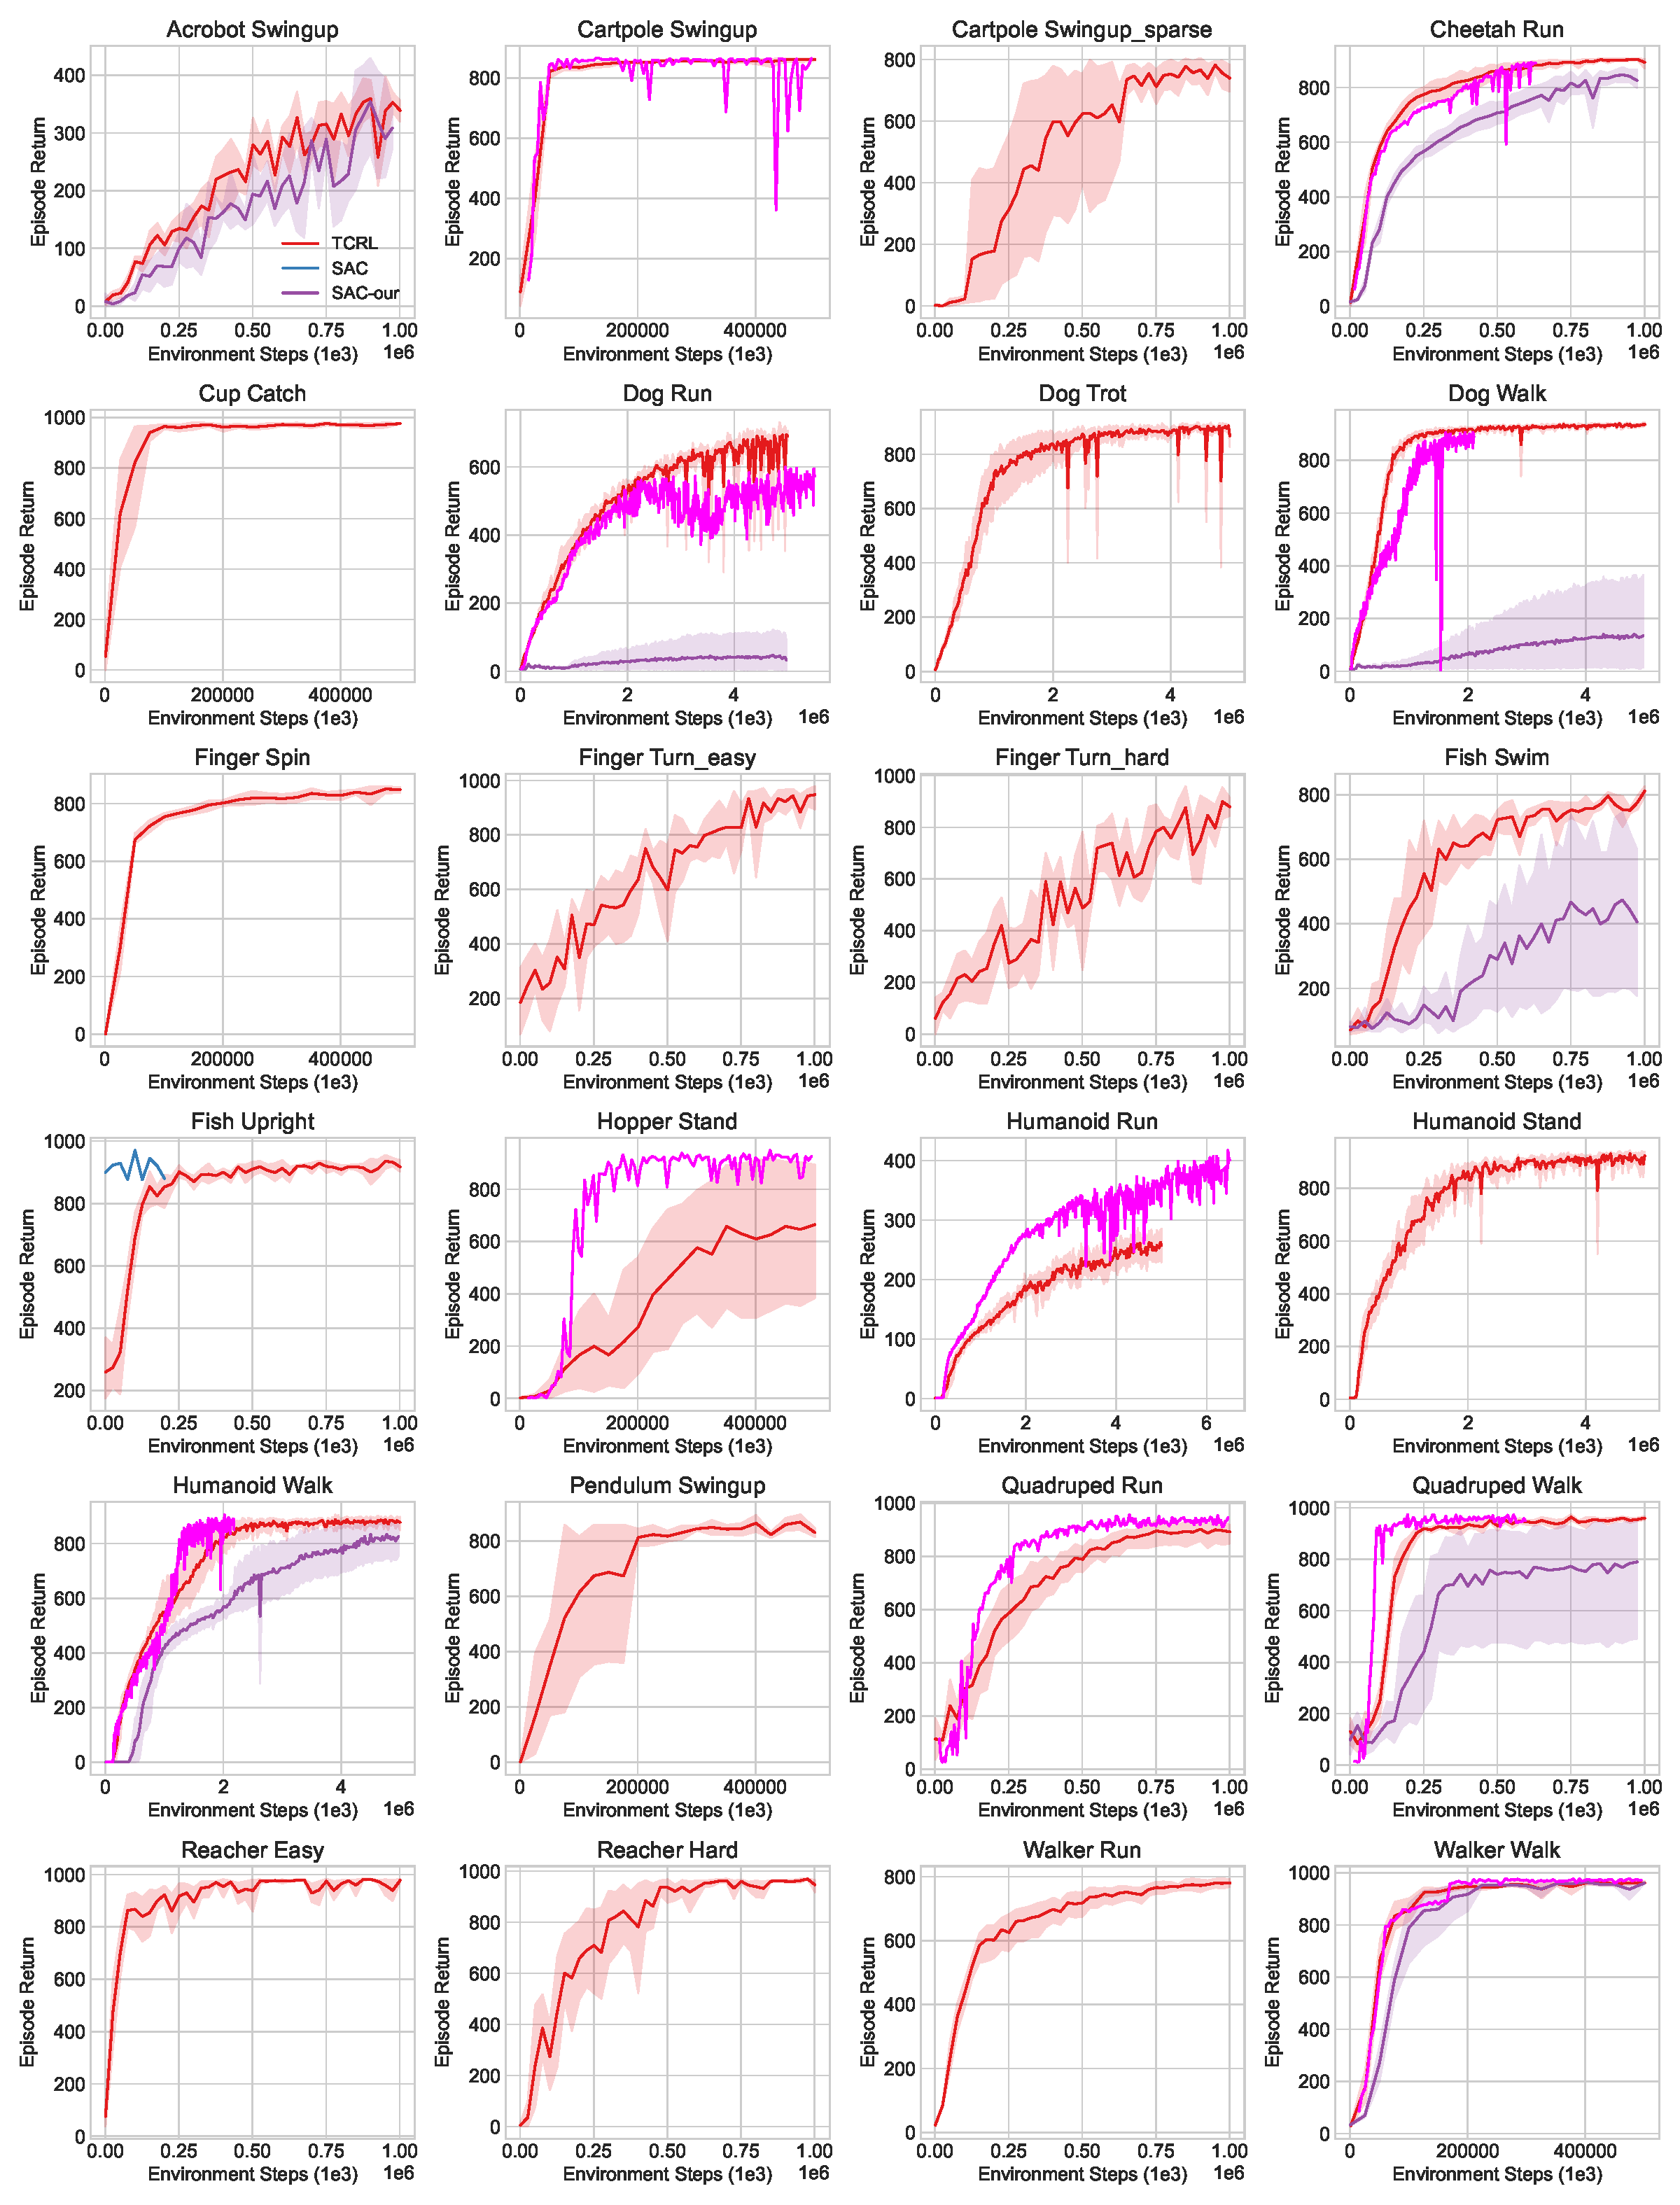
\includegraphics[width=0.97\textwidth]{./figs/all_mujoco_envs.pdf}}
\caption{Comparison to SAC/TCRL with UTD=1.}
\label{fig:main_plot}
\end{center}
\vskip -0.2in
\end{figure*}
%%%%%%%%%%%%%%%%%%%%%%%%%%%%%%%%%%%%%%%%%%%%%%%%%%%%%%%%%%%%%%%%%%%%%%%%%%%%%%%
%%%%%%%%%%%%%%%%%%%%%%%%%%%%%%%%%%%%%%%%%%%%%%%%%%%%%%%%%%%%%%%%%%%%%%%%%%%%%%%


\end{document}


% This document was modified from the file originally made available by
% Pat Langley and Andrea Danyluk for ICML-2K. This version was created
% by Iain Murray in 2018, and modified by Alexandre Bouchard in
% 2019 and 2021 and by Csaba Szepesvari, Gang Niu and Sivan Sabato in 2022.
% Modified again in 2023 and 2024 by Sivan Sabato and Jonathan Scarlett.
% Previous contributors include Dan Roy, Lise Getoor and Tobias
% Scheffer, which was slightly modified from the 2010 version by
% Thorsten Joachims & Johannes Fuernkranz, slightly modified from the
% 2009 version by Kiri Wagstaff and Sam Roweis's 2008 version, which is
% slightly modified from Prasad Tadepalli's 2007 version which is a
% lightly changed version of the previous year's version by Andrew
% Moore, which was in turn edited from those of Kristian Kersting and
% Codrina Lauth. Alex Smola contributed to the algorithmic style files.
